% Symmetries of the plane
% Author: Cristóbal Camarero Coterillo
\documentclass[a4paper, 12pt, landscape]{article}
\usepackage[utf8]{inputenc}
\usepackage{textcomp}
\usepackage{tikz}
%%%<
\usepackage{verbatim}
%%%>
\begin{comment}
:Title: Symmetries of the plane
:Tags: Foreach;Mathematics
:Author: Cristóbal Camarero Coterillo
:Slug: symmetries
\end{comment}
\usetikzlibrary{shapes,calc,decorations.pathmorphing,decorations.fractals}
\usepackage[bookmarks=true]{hyperref}

%landscape tuning
\setlength{\oddsidemargin}{0in}		% default=0in
\setlength{\textwidth}{9in}		% default=9in
\setlength{\columnsep}{0.5in}		% default=10pt
\setlength{\columnseprule}{1pt}		% default=0pt (no line)
\setlength{\textheight}{5.85in}		% default=5.15in
\setlength{\topmargin}{-0.15in}		% default=0.20in
\setlength{\headsep}{0.25in}		% default=0.35in
\setlength{\parskip}{1.2ex}
\setlength{\parindent}{0mm}

%PDF Settings
\newcommand\titulo{Symmetries of the plane}
\newcommand\autor{\href{http://www.alumnos.unican.es/ccc66}
  {Cristóbal Camarero Coterillo}}
\hypersetup{
    %bookmarks=true,         % show bookmarks bar?
    unicode=false,          % non-Latin characters in Acrobats bookmarks
    pdftoolbar=true,        % show Acrobats toolbar?
    pdfmenubar=true,        % show Acrobats menu?
    pdffitwindow=true,      % page fit to window when opened
    pdftitle={\titulo},     % title
    pdfauthor={\autor},     % author
    pdfsubject={symmetries of the plane in tikz},	% subject of the document
    pdfnewwindow=true,      % links in new window
    pdfkeywords={plane,symmetry,orbifold},% list of keywords
	pdfpagemode=None,		% avoid auto open bookmarks
    colorlinks=false,       % false: boxed links; true: colored links
    linkcolor=red,          % color of internal links
    citecolor=green,        % color of links to bibliography
    filecolor=magenta,      % color of file links
    urlcolor=cyan           % color of external links
}

\begin{document}
%%%<
\title{\titulo}
\author{\autor}
\date{}
\maketitle%

An implementation of all 17 plane symmetries in Ti\textit{k}Z.
With the orbifold signature these are the following:

\[\color{red}
\begin{array}{ccccc}
*632				&	*442					&	*333					&	*2222					&	**	\\
					&							&							&	{\color{blue}2}\!*\!22	&	*\times\\
					&	{\color{blue}4}\!*\!2	&	{\color{blue}3}\!*\!3	&	{\color{blue}22}*		&		\\
					&							&							&	{\color{blue}22}\times	&\times\times\\
{\color{blue}632}	&	{\color{blue}442}		&	{\color{blue}333}		&	{\color{blue}2222}		&	{\color{blue}\circ}\\
\end{array}
\]

For their meaning and more pretty pictures see \textit{``The Symmetries of Things''}
by John H. Conway, Heidi Burgiel and Chaim Goodman-Strauss.\\

A brief comment about the orbifold signature:
A number $\color{blue}n$ before $\color{red}*$ represent a \textbf{gyration
point} of order $n$, thus in $\color{blue}632$ we have three effectively
distinct points with respective orders 6, 3 and 2.  Each $\color{red}*$
represent a kaleidoscope, a kaleidoscope which is not followed by a number is a
mirror, a following number $\color{red}n$ represent a point where $n$
\textbf{mirror lines} cross.  Thus, in $\color{red}*333$ we have a kaleidoscope
with 3 different points, in each one, there are crossing 3 mirrors.  In
$\color{blue}4\!\color{red}*\!2$ we have a gyration point of order 4, the four
neighbour point are actually the same point, a point where 2 mirrors cross.
The $\color{red}\times$ is called a \textbf{miracle} and represent a reflection
which cannot be explained by a mirror line.  Finally, the $\color{blue}\circ$
is called a \textbf{wonder} and represents translations which
are not explained by any previous symbol.
%%%>

\newsavebox{\piece}%A TeX box to store the base tile (or orbifold)
\clearpage

%*632
\phantomsection\addcontentsline{toc}{chapter}{*632}%Add to PDF bookmarks
\savebox{\piece}{%We create the base tile
\begin{tikzpicture}[overlay]
\node[star,draw=red!50!black,inner sep=1pt] at (0.7,0.3) {};
\node[red,anchor=base] at (0.55,0.05) {\tiny $*632$};
\draw[thin] (0,0) -- ++(0:1) -- ++(120:0.5) --cycle;
\end{tikzpicture}}
\begin{center}%We replicate the tile according to the symmetry
\begin{tikzpicture}[every node/.style={anchor=center,draw=none}]
%The \i loop creates a supertile which can tile by translations
%which is done by the \a and \b loops
	\foreach \a in {0,...,7}
	\foreach \b in {0,...,7}
	\foreach \i in {0,1,2,3,4,5}
	{
		\path (0,0)
			++(0:\a) ++(60:\a) ++(0:\b) ++(-60:\b)
			node[rotate=\i*60] {\usebox{\piece}}
			node[rotate=\i*60,yscale=-1] {\usebox{\piece}};
	}
\end{tikzpicture}
\end{center}
\clearpage

%632
\phantomsection\addcontentsline{toc}{chapter}{632}
\savebox{\piece}{%
\begin{tikzpicture}[overlay]
\node[blue] at (0.3,0.4) {\tiny 632};
\draw[thin] (0,0) -- ++(0:1) -- ++(120:1) --cycle;
\end{tikzpicture}}
\begin{center}
\begin{tikzpicture}[every node/.style={anchor=center,draw=none}]
	\foreach \a in {0,...,8}
	\foreach \b in {0,...,8}
	\foreach \i in {0,1,2,3,4,5}
	{
		\path (0,0)
			++(0:\a) ++(60:\a) ++(0:\b) ++(-60:\b)
			node[rotate=\i*60] {\usebox{\piece}};
	}
\end{tikzpicture}
\end{center}
\clearpage

%*442
\phantomsection\addcontentsline{toc}{chapter}{*442}
\savebox{\piece}{%
\begin{tikzpicture}[overlay]
\node[arrow box,arrow box arrows={south:0.5cm,west:0.5cm},draw=red!50!black,inner sep=4pt] at (0.8,0.8) {};
\node[red,anchor=base] at (0.4,0.05) {\tiny $*442$};
\draw[thin] (0,0) -- ++(0:1) -- ++(90:1) --cycle;
\end{tikzpicture}}
\begin{center}
\begin{tikzpicture}[every node/.style={anchor=center,draw=none}]
	\foreach \a in {0,...,8}
	\foreach \b in {0,...,7}
	\foreach \i in {0,1,2,3}
	{
		\path (0,0) ++(0:2*\a) ++(90:2*\b)
			node[rotate=\i*90] {\usebox{\piece}}
			node[rotate=\i*90,yscale=-1] {\usebox{\piece}};
	}
\end{tikzpicture}
\end{center}
\clearpage

%4*2
\phantomsection\addcontentsline{toc}{chapter}{4*2}
\savebox{\piece}{%
\begin{tikzpicture}[overlay]
\node[single arrow,draw,shape border rotate=90,inner sep=0pt,minimum height=.5cm] at (0.5,0.6) {\tiny up};
\node[blue] at (0.3,0.3) {\tiny 4\color{red}$*$2};
\draw[thin] (0,0) -- ++(0:1) -- ++(90:1) -- ++(180:1) --cycle;
\end{tikzpicture}}
\begin{center}
\begin{tikzpicture}[every node/.style={anchor=center,draw=none}]
	\foreach \a in {0,...,4}
	\foreach \b in {0,...,3}
	\foreach \i in {0,1,2,3}
	{
		\path (0,0) ++(0:4*\a) ++(90:4*\b)
			node[rotate=\i*90] {\usebox{\piece}}
			+(2,0) node[rotate=\i*90,xscale=-1] {\usebox{\piece}}
			+(0,2) node[rotate=\i*90,yscale=-1] {\usebox{\piece}}
			+(2,2) node[rotate=\i*90] {\usebox{\piece}};
	}
\end{tikzpicture}
\end{center}
\clearpage

%442
\phantomsection\addcontentsline{toc}{chapter}{442}
\savebox{\piece}{%
\begin{tikzpicture}[overlay]
\node[blue] at (0.3,0.4) {\tiny 442};
\draw[red!40!green] (1,0) -- (14/29,35/29);
\draw[densely dotted,red] (14/29,35/29) -- (1,1);
\draw[thin] (0,0) -- ++(0:1) -- ++(90:1) -- ++(180:1) --cycle;
\end{tikzpicture}}
\begin{center}
\begin{tikzpicture}[every node/.style={anchor=center,draw=none}]
	\foreach \a in {0,...,8}
	\foreach \b in {0,...,6}
	\foreach \i in {0,1,2,3}
	{
		\path (0,0) ++(0:2*\a) ++(90:2*\b)
			node[rotate=\i*90] {\usebox{\piece}};
	}
\end{tikzpicture}
\end{center}
\clearpage

%*333
\phantomsection\addcontentsline{toc}{chapter}{*333}
\savebox{\piece}{%
\begin{tikzpicture}[overlay]
\node[regular polygon,regular polygon sides=3,draw=green,inner sep=2pt] at (0.5,0.55) {};
\node[red] at (0.45,0.2) {\tiny $*333$};
\draw[thin] (0,0) -- ++(0:1) -- ++(120:1) --cycle;
\end{tikzpicture}}
\begin{center}
\begin{tikzpicture}[every node/.style={anchor=center,draw=none}]
	\foreach \a in {0,...,8}
	\foreach \b in {0,...,7}
	\foreach \i in {0,1,2}
	{
		\path (0,0)
			++(0:\a) ++(60:\a) ++(0:\b) ++(-60:\b)
			node[rotate=\i*120] {\usebox{\piece}}
			node[rotate=\i*120-60,xscale=-1] {\usebox{\piece}};
	}
\end{tikzpicture}
\end{center}
\clearpage

%3*3
\phantomsection\addcontentsline{toc}{chapter}{3*3}
\pgfmathparse{sqrt(3)/3}
\let\altitude=\pgfmathresult
\savebox{\piece}{%
\begin{tikzpicture}[overlay]
\node[blue] at (0,-0.2) {\tiny 3\color{red}$*$3};
\draw[thin,decorate,decoration={coil,amplitude=.5pt,segment length=0.5*\altitude cm}] (0,0) -- ++(-30:\altitude);
\draw[thin,dashed] (0,0) ++(-30:\altitude) -- ++(-1,0);
\end{tikzpicture}}
\begin{center}
\begin{tikzpicture}[every node/.style={anchor=center,draw=none}]
	\foreach \a in {0,...,11}
	\foreach \b in {0,...,12}
	\foreach \i in {0,1,2}
	{
		\path (0,0)
			++(90:\a*\altitude) ++(30:\a*\altitude) ++(-30:\b*\altitude) ++(30:\b*\altitude)
			node[rotate=\i*120] {\usebox{\piece}}
			+(0,-\altitude) node[rotate=\i*120,yscale=-1] {\usebox{\piece}};
	}
\end{tikzpicture}
\end{center}
\clearpage

%333
\phantomsection\addcontentsline{toc}{chapter}{333}
\savebox{\piece}{%
\begin{tikzpicture}[overlay]
\draw[red] (0.2,0.17) circle (2pt);
\draw[blue] (0.6,0.3) circle (3pt);
\node at (-0.1,0.5) {p};
\node[blue] at (0.3,0.7) {\tiny 333};
\draw[thick] (0,0) -- ++(0:1) -- ++(120:1) -- ++(180:1) --cycle;
\end{tikzpicture}}
\begin{center}
\begin{tikzpicture}[every node/.style={anchor=center,draw=none}]
	\foreach \a in {0,...,8}
	\foreach \b in {0,...,8}
	\foreach \i in {0,1,2}
	{
		\path (0,0) ++(0:\a) ++(60:\a) ++(0:\b) ++(-60:\b)
			node[rotate=\i*120] {\usebox{\piece}};
	}
\end{tikzpicture}
\end{center}
\clearpage

%*2222
\phantomsection\addcontentsline{toc}{chapter}{*2222}
\savebox{\piece}{%
\begin{tikzpicture}[overlay]
\node[arrow box,arrow box arrows={south:0.5cm,west:0.5cm},draw=red!50!black,inner sep=4pt] at (0.8,0.8) {};
\node[red] at (0.3,0.4) {\tiny $*2222$};
\draw[thin] (0,0) -- ++(0:1) -- ++(90:1) -- ++(180:1) --cycle;
\end{tikzpicture}}
\begin{center}
\begin{tikzpicture}[every node/.style={anchor=center,draw=none}]
	\foreach \a in {0,...,9}
	\foreach \b in {0,...,7}
	\foreach \i in {0,1}
	{
		\path (0,0) ++(0:2*\a) ++(90:2*\b)
			node[rotate=\i*180] {\usebox{\piece}}
			node[rotate=\i*180,yscale=-1] {\usebox{\piece}};
	}
\end{tikzpicture}
\end{center}
\clearpage

%2*22
\phantomsection\addcontentsline{toc}{chapter}{2*22}
\savebox{\piece}{%
\begin{tikzpicture}[overlay]
\node[blue] at (0.0,0.4) {\tiny 2\color{red}$*$22};
\draw[very thin,red,densely dotted] (0,0) ++(0:0.5) -- ++(90:1) -- ++(180:1) -- ++(-90:1);
\draw[very thick,decoration=Cantor set] (0,0) decorate{decorate{++(0:0.5) -- ++(90:1) -- ++(180:1) -- ++(-90:1)}};
\draw[thin,decoration=Koch curve type 2,color=blue!60!black] decorate{decorate{decorate{(-0.5,0)--(0.5,0)}}};
\end{tikzpicture}}
\begin{center}
\begin{tikzpicture}[every node/.style={anchor=center,draw=none}]
	\foreach \a in {0,...,8}
	\foreach \b in {0,...,3}
	\foreach \i in {0,1}
	{
		\path (0,0) ++(0:2*\a) ++(90:4*\b)
			node[rotate=\i*180] {\usebox{\piece}}
			+(0,2) node[rotate=\i*180,yscale=-1] {\usebox{\piece}}
			+(1,0) node[rotate=\i*180,xscale=-1] {\usebox{\piece}}
			+(1,2) node[rotate=\i*180] {\usebox{\piece}};
	}
\end{tikzpicture}
\end{center}
\clearpage

%22*
\phantomsection\addcontentsline{toc}{chapter}{22*}
\savebox{\piece}{%
\begin{tikzpicture}[overlay]
\node[blue,anchor=base east] at (0.5,0.05) {\tiny 22\color{red}$*$};
\draw[thick,blue,rounded corners] (0,0.2) -- ++(0.4,0.3) -- ++(-0.8,0.3) --(0,1);
\draw[thin] (0,0) -- ++(0:0.5) -- ++(90:1) -- ++(180:1) -- ++(-90:1) --cycle;
\fill[red] (-0.5,0.6) arc[start angle=90,end angle=-90,x radius=0.2cm,y radius=0.3cm];
\fill[red] (0.5,0.6) arc[start angle=-90,end angle=90,x radius=0.17cm,y radius=0.21cm];
\end{tikzpicture}}
\begin{center}
\begin{tikzpicture}[every node/.style={anchor=center,draw=none}]
	\foreach \a in {0,...,8}
	\foreach \b in {0,...,6}
	\foreach \i in {0,1}
	{
		\path (0,0) ++(0:2*\a) ++(90:2*\b)
			node[rotate=\i*180] {\usebox{\piece}}
			+(1,0) node[rotate=\i*180,xscale=-1] {\usebox{\piece}};
	}
\end{tikzpicture}
\end{center}
\clearpage

%22x
\phantomsection\addcontentsline{toc}{chapter}{22\texttimes}
\def\miraclelength{0.3}
\savebox{\piece}{%
\begin{tikzpicture}[overlay]
\node[blue,anchor=base east] at (0.5,0.05) {\tiny 22\color{red}$\times$};
\draw[thick,blue,rounded corners] (0,0.2) -- (0.4,0.5) -- (-0.4,0.4) --(0,1);
\draw[thick,dashdotted,red!50!black] (0,0) ++(0:0.5) -- ++(90:1);
\fill[red] (.1,0.7) circle (0.15cm);
\end{tikzpicture}}
\begin{center}
\begin{tikzpicture}[every node/.style={anchor=center,draw=none}]
	\foreach \a in {0,...,8}
	\foreach \b in {0,...,6}
	\foreach \i in {0,1}
	{
		\path (0,0) ++(0:2*\a) ++(90:2*\b)
			node[rotate=\i*180] {\usebox{\piece}}
			+(1,\miraclelength) node[rotate=\i*180,xscale=-1] {\usebox{\piece}};
	}
\end{tikzpicture}
\end{center}
\clearpage

%2222
\phantomsection\addcontentsline{toc}{chapter}{2222}
\savebox{\piece}{%
\begin{tikzpicture}[overlay]
\node[blue,anchor=base east] at (0.5,0.05) {\tiny 2222};
\draw[thick,blue,rounded corners] (0,0.2) -- ++(0.4,0.3) -- ++(-0.8,0.3) --(0,1);
\draw[draw=gray,double={blue!50!green},rounded corners] (-0.5,0.5) -- (-0.3,0.3) -- (0.3,0.8) -- (0.5,0.5);
\end{tikzpicture}}
\begin{center}
\begin{tikzpicture}[every node/.style={anchor=center,draw=none}]
	\foreach \a in {0,...,8}
	\foreach \b in {0,...,6}
	\foreach \i in {0,1}
	{
		\pgfmathparse{-(-1)^\i}
		\let\res=\pgfmathresult
		\path (0,0) ++(0:2*\a) ++(90:2*\b)
			node[rotate=\i*180] {\usebox{\piece}}
			+(1,\res) node[rotate=\i*180] {\usebox{\piece}};
	}
\end{tikzpicture}
\end{center}
\clearpage

%**
\phantomsection\addcontentsline{toc}{chapter}{**}
\def\repetition{1.0}
\savebox{\piece}{%
\begin{tikzpicture}[overlay]
\node[red,draw=red!80!black,shape=rectangle callout,anchor=center] at (0.5,0.5) {\tiny **};
\end{tikzpicture}}
\begin{center}
\begin{tikzpicture}[every node/.style={anchor=center,draw=none}]
	\foreach \a in {0,...,8}
	\foreach \b in {0,...,12}
	\foreach \i in {0,1}
	{
		\path (0,0) ++(0:2*\a) ++(90:\b*\repetition)
			node {\usebox{\piece}}
			node[xscale=-1] {\usebox{\piece}};
	}
\end{tikzpicture}
\end{center}
\clearpage

%*x
\phantomsection\addcontentsline{toc}{chapter}{*\texttimes}
\def\repetition{2.0}
\def\miraclelength{0.5}
\savebox{\piece}{%

\begin{tikzpicture}[overlay]
\draw[red,fill=red!10,rounded corners] (0,0) -- (1.0,1.0) arc[start angle=0,end angle=180,x radius=0.5cm,y radius=0.5cm];
\node[red,anchor=base west] at (0.1,0.7) {\small $*\times$};
\end{tikzpicture}}
\begin{center}
\begin{tikzpicture}[every node/.style={anchor=center,draw=none}]
	\foreach \a in {0,...,7}
	\foreach \b in {0,...,5}
	\foreach \i in {0,1}
	{
		\path (0,0) ++(2*\a,\miraclelength*\a) ++(90:\b*\repetition)
			node {\usebox{\piece}}
			node[xscale=-1] {\usebox{\piece}};
	}
\end{tikzpicture}
\end{center}
\clearpage

%xx
\phantomsection\addcontentsline{toc}{chapter}{\texttimes\texttimes}
\def\repetition{2.0}
\def\miraclelength{0.5}
\savebox{\piece}{%
\begin{tikzpicture}[overlay]
\draw[green,thick] (1.0,0.5) -- (0.3,0) (1.0,0.5) -- (0.8,0) (1.3,0.0) -- (1.55,0.2) -- (1.8,0.0);
\node[draw,shape=starburst,red,starburst point height=0.3cm,inner sep=0pt] at (1.0,0.5) {\small $\times\times$};
\end{tikzpicture}}
\begin{center}
\begin{tikzpicture}[every node/.style={anchor=center,draw=none}]
	\foreach \a in {0,...,7}
	\foreach \b in {0,...,5}
	{
		\path (0,0) ++(0:\repetition*\a) ++(90:2*\b)
			node {\usebox{\piece}}
			+(0:\miraclelength) node[yscale=-1] {\usebox{\piece}};
	}
\end{tikzpicture}
\end{center}
\clearpage

%o
\phantomsection\addcontentsline{toc}{chapter}{o}
\def\repetitionax{1.0}
\def\repetitionay{0.2}
\def\repetitionbx{0.5}
\def\repetitionby{2.0}
\pgfmathparse{0.5*(\repetitionax+\repetitionbx)}
\let\repetitioncx=\pgfmathresult
\pgfmathparse{0.5*(\repetitionay+\repetitionby)}
\let\repetitioncy=\pgfmathresult
\savebox{\piece}{%

\begin{tikzpicture}[overlay]
\node[blue,anchor=center] at (\repetitioncx,\repetitioncy) {\small $\circ$};
\fill[blue!80!black] (0,0) circle (0.3cm);
\fill[blue!80] (0.5,0.4) circle (0.2cm);
\fill[blue!40!green] (0.2,0.8) circle (0.25cm);
\fill[blue!60!red] (0.6,1.5) circle (0.15cm);
\end{tikzpicture}}
\begin{center}
\begin{tikzpicture}[every node/.style={anchor=center,draw=none}]
	\foreach \a in {0,...,14}
	\foreach \b in {0,...,5}
	{
		\path (0,0) ++(\repetitionax*\a,\repetitionay*\a) ++(\repetitionbx*\b,\repetitionby*\b)
			node {\usebox{\piece}};
	}
\end{tikzpicture}
\end{center}
\clearpage
\end{document}

